\section{Development Process and Team Collaboration}

This section explains how a two-person team organized design, implementation, and validation, and how version control and shared build conventions kept the codebase consistent across machines.

\subsection{Development timeline and phases}
Work proceeded in four overlapping phases. The boundaries were not strictly sequential—for example, tests were added alongside features—but the phases help explain how risk was managed.

\begin{table}[htbp]
    \centering
    \small
    \caption{High-level development phases and concrete artifacts.}
    \label{tab:dev_phases}
    \begin{tabularx}{\textwidth}{@{}l X X@{}}
        \toprule
        \textbf{Phase} & \textbf{Focus} & \textbf{Representative artifacts} \\
        \midrule
        Design &
        Agree on module boundaries, configuration schema, compressed-container layout, and error-handling style (typed return codes). &
        Headers under \url{include/}; early stubs in \url{src/parsers/}, \url{src/components/}, \url{src/compressions/}. \\
        \addlinespace
        Parallel implementation &
        Implement parsers, engine orchestration, ASCII rendering, compression algorithms, and preview consumption along separate but stable interfaces. &
        \url{src/parsers/json/config.c}, \url{src/components/engine.c}, \url{src/compressions/}, \url{src/components/preview.c}. \\
        \addlinespace
        Integration &
        Connect engine output to compression and logging; align config keys (e.g.\ \texttt{compression\_algorithm}, optional \texttt{huffman\_K}) with runtime behavior. &
        \url{src/components/render_compress.c}, \url{output/demo/demo_engine/}. \\
        \addlinespace
        Validation &
        Run unit tests per module; exercise end-to-end runs with demo configs and inspect \url{output/} logs and renders. &
        \url{tests/}, \url{Makefile} targets \texttt{test} / \texttt{run\_test}. \\
        \bottomrule
    \end{tabularx}
\end{table}

\subsection{Work split for a two-person team}
The project naturally splits into a \textbf{media ingestion and orchestration track} and a \textbf{compression and delivery track}. Both tracks are required for the product narrative (correct rendering \emph{and} usable compressed output with preview).

\begin{itemize}
    \item \textbf{Subsystem A — parsers, engine, and raw rendering.} One teammate focused on JSON configuration loading and validation, WAV and BMP parsing, frame sequencing, the engine state machine, ASCII conversion, plain-text render output, and process logging. This track establishes the functional contract: what a ``frame'' means, how audio lines up with frames, and what the uncompressed render records look like.
    \item \textbf{Subsystem B — compression, decompression, and preview.} The other teammate focused on algorithm implementations (including symbol statistics and Huffman table/FSM preparation where applicable), the compressed file format, \url{compress_frame}/\url{decompress_frame} integration, and the terminal preview path that reads headers and frame payloads. This track delivers storage-efficient artifacts and user-facing playback.
\end{itemize}

\textbf{Shared ownership.} Interface decisions (e.g.\ fields in \url{include/parsers/json/config.h}, structures in \url{include/components/render_compress.h}) and naming conventions were agreed explicitly so that changes on one side did not silently break the other. End-to-end behavior was validated together using shared demo inputs under \url{output/demo/}.

\subsection{Version control with GitHub}
We used \textbf{Git} with a \textbf{GitHub} remote as the single source of truth. This choice supported parallel development with minimal merge pain:

\begin{itemize}
    \item \textbf{Isolated changes:} Work on parsers/engine and on compression/preview touched mostly disjoint file trees (\url{src/parsers/}, \url{src/components/engine.c} \emph{vs.}\ \url{src/compressions/}, \url{src/components/preview.c}), which reduced the chance of conflicting edits in the same region of a file.
    \item \textbf{Small, reviewable steps:} Features were integrated through the shared remote using direct pushes to a main \textbf{integration branch} (exact branching policy is a team convention; the important point is that history remained centralized and inspectable).
    \item \textbf{Traceability:} Commit messages and pull requests (when used) document \emph{what} changed and \emph{why}, which complements the process log produced at runtime by the engine.
\end{itemize}

GitHub did not replace local validation: every integration still had to compile and pass targeted tests on each machine (\S\ref{sec:repro_team}).

\subsection{Integration strategy and interface contracts}
Integration risk was concentrated at a few well-defined boundaries:

\begin{enumerate}[label=\arabic*)]
    \item \textbf{Configuration $\rightarrow$ engine.} The JSON schema enforced by \url{config_load} (\url{src/parsers/json/config.c}) determines frame paths, timing parameters, palette, threshold, and compression mode. Invalid or unknown keys fail early, which avoids partial runs with ambiguous state.
    \item \textbf{ASCII frame $\rightarrow$ compression.} The engine produces structured ASCII output and passes frame payloads into the compression layer through the shared types declared in \url{include/components/render_compress.h} and \url{include/compressions/compress.h}. Agreement on width/height, compression enum, and Huffman parameters (\texttt{huffman\_K}) was essential for round-trip correctness.
    \item \textbf{Compressed file $\rightarrow$ preview.} The preview program (\url{src/components/preview.c}) must parse the same textual header markers and binary frame layout that the writer emits. Any change to the on-disk format required coordinated updates on both sides.
\end{enumerate}

When integration issues appeared (e.g.\ mismatched frame naming or compression strings), we used \textbf{reproducible demo configs} and \textbf{diffs in Git} to locate whether the fault lay in parsing, engine logic, or the codec path.

\begin{figure}[htbp]
    \centering
    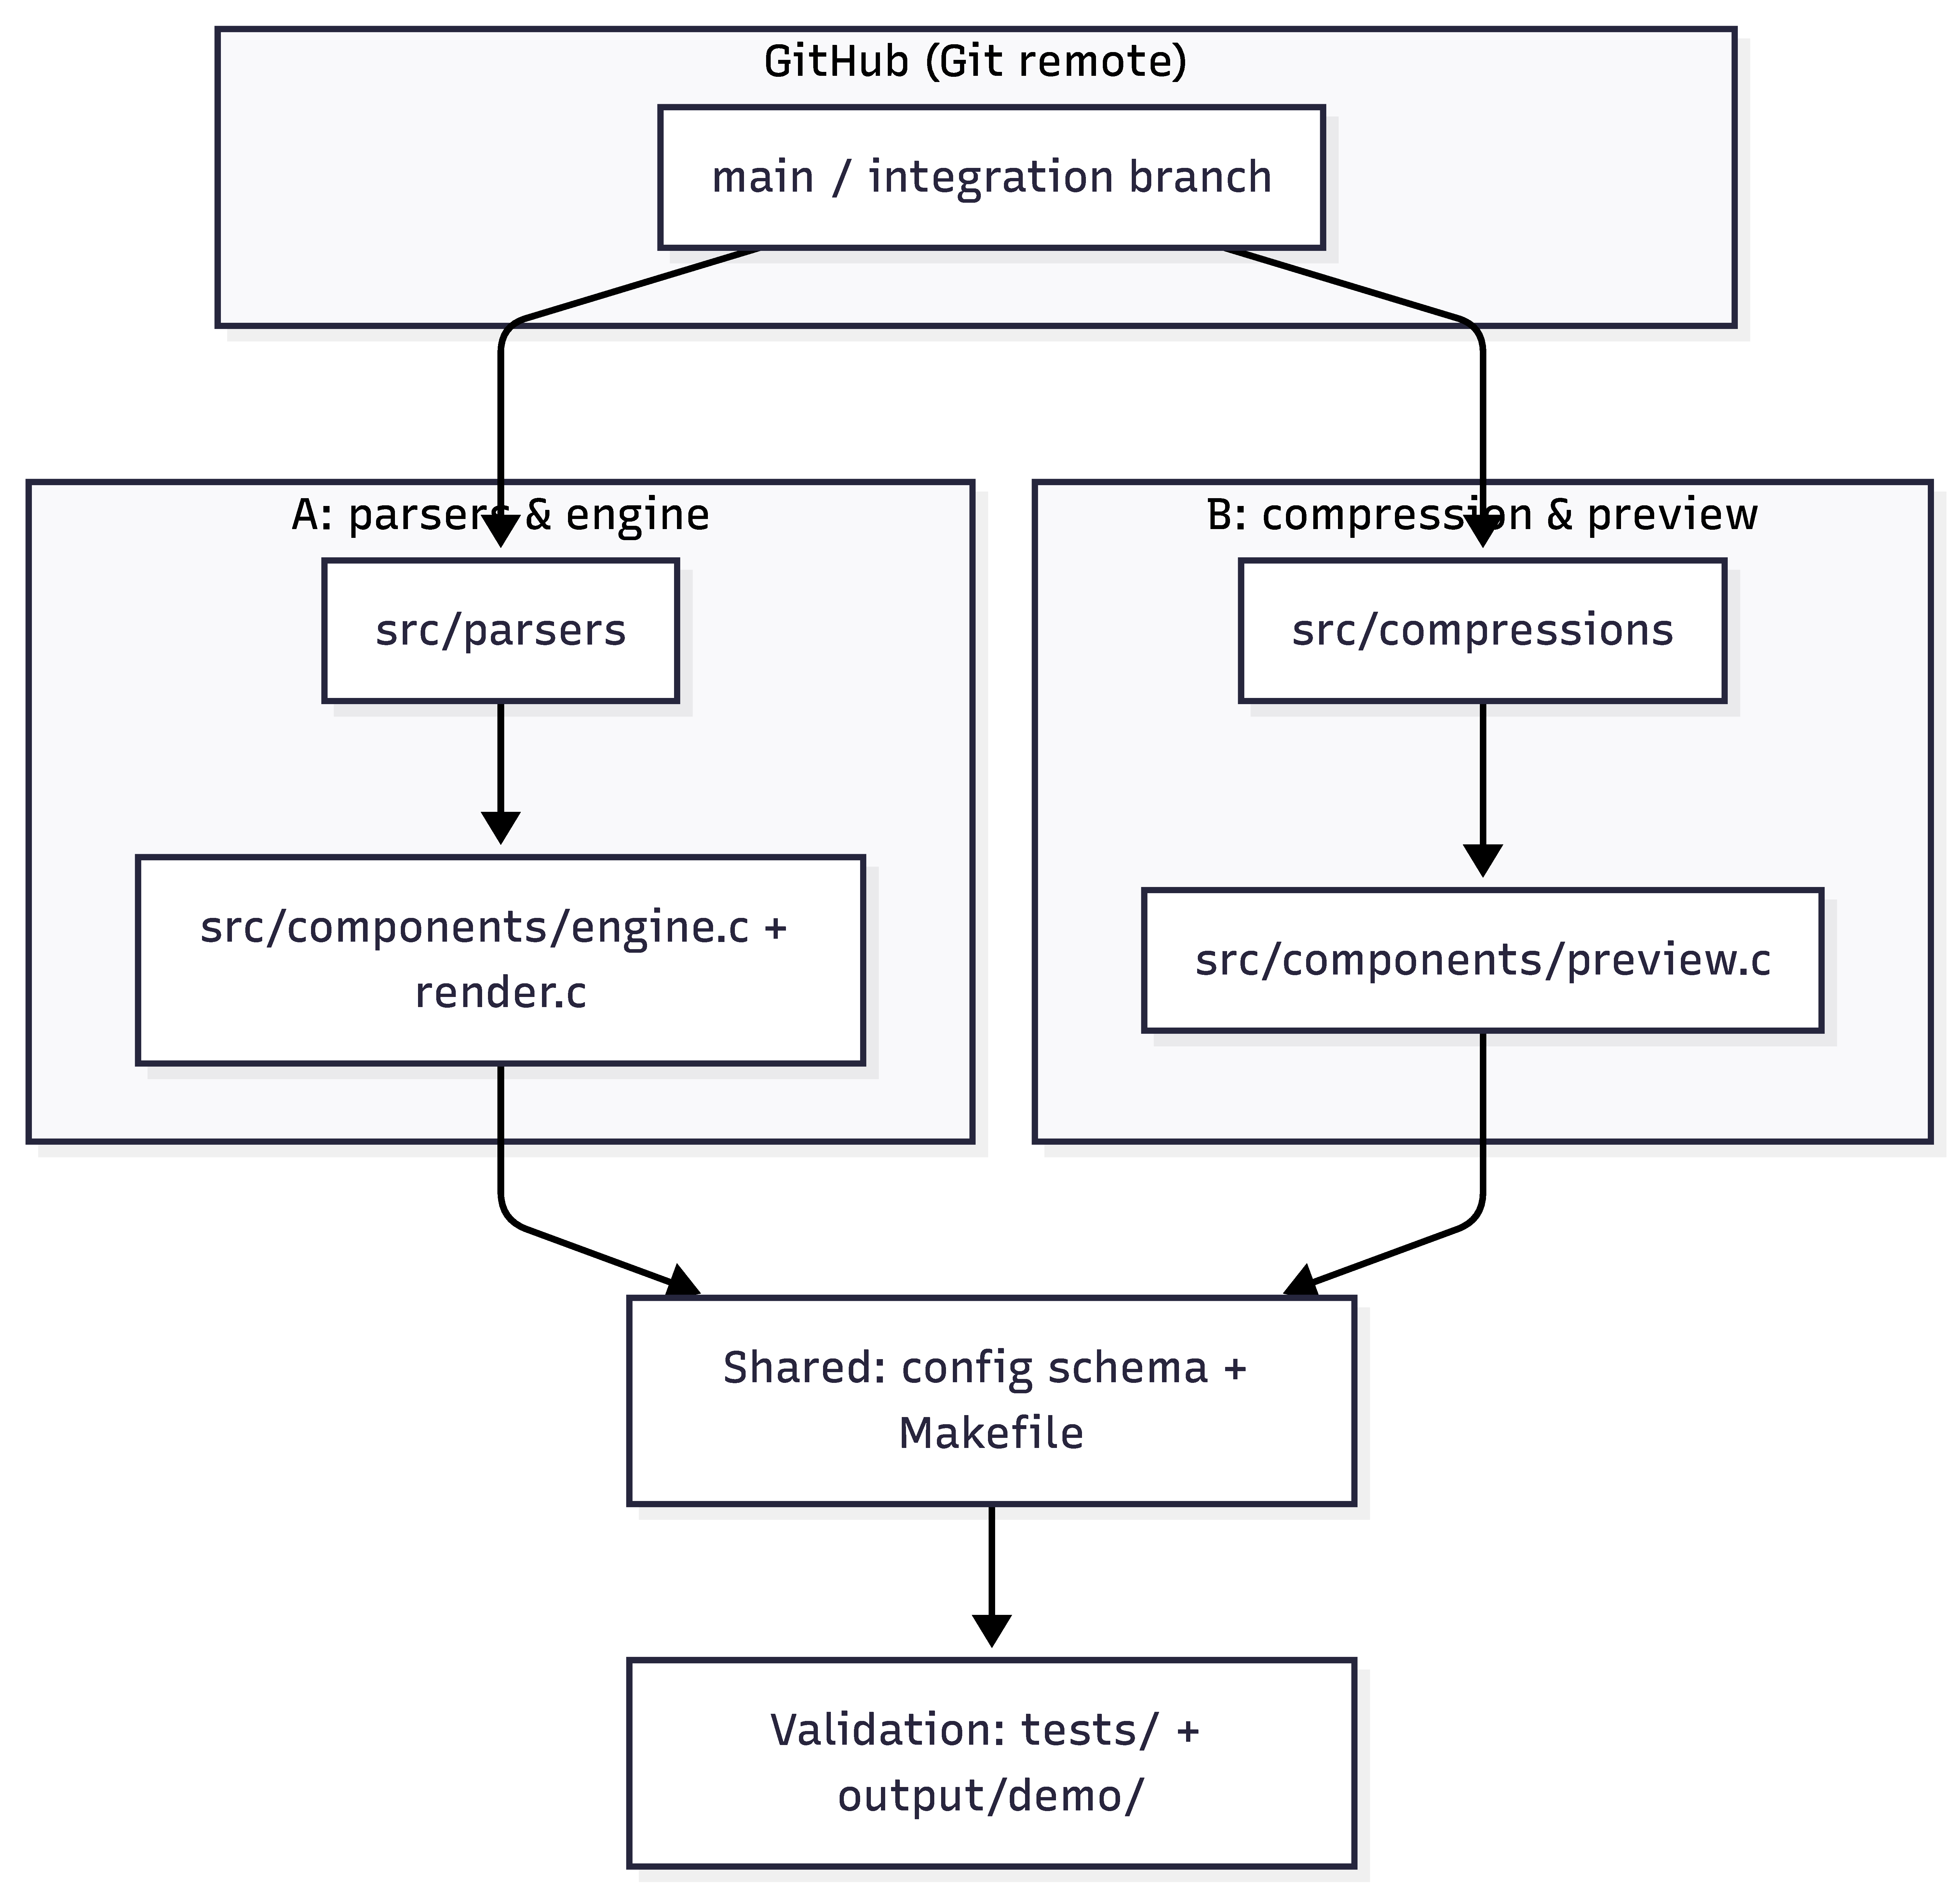
\includegraphics[width=0.55\textwidth]{figures/team_workstream.pdf}
    \caption{Parallel workstreams converging on shared contracts and a Makefile-driven build.}
    \label{fig:collab_overview}
\end{figure}

% \begin{verbatim}
% flowchart TB
%   subgraph Remote["GitHub (Git remote)"]
%     R[main / integration branch]
%   end
%   subgraph A["A: parsers & engine"]
%     A1[src/parsers]
%     A2[src/components/engine.c + render.c]
%   end
%   subgraph B["B: compression & preview"]
%     B1[src/compressions]
%     B2[src/components/preview.c]
%   end
%   R --> A1 --> A2
%   R --> B1 --> B2
%   A2 --> C[Shared: config schema + Makefile]
%   B2 --> C
%   C --> V[Validation: tests/ + output/demo/]
% \end{verbatim}

\subsection{Reproducibility across team machines}
\label{sec:repro_team}

\textbf{Build system.} The project is built with \texttt{make} from a root \url{Makefile}. Compiler flags (\texttt{-Wall -Werror -ansi -pedantic -Iinclude}) apply uniformly, so a warning on one laptop is a warning for everyone. Targets such as \texttt{retrovision} and \texttt{preview} encode the link line and object lists, reducing ``works on my machine'' drift.

\noindent \textbf{Tests.} Unit tests live under \url{tests/} and are compiled on demand, e.g.\ \texttt{make run\_test TEST=tests/parsers/test\_wav.c}. Sharing a small set of \emph{known-good} test invocations in chat meant both members verified the same behavior before merging.

\noindent \textbf{Demo artifacts.} The \url{output/demo/} tree (including \url{output/demo/demo_engine/}) provides sample configs, logs, and outputs for cross-checking integration. Comparing \url{process.log} and compressed outputs after a merge quickly surfaces regressions.

\noindent \textbf{Environment assumptions.} Both sides used a standard C toolchain (\texttt{gcc}) and POSIX-style shells; preview code accounts for Windows vs.\ POSIX timing (\url{src/components/preview.c}). No external dependency manager was required, which simplified onboarding.
